Die in dieser Arbeit vorgestellten Methoden wurden auf reale chemische Fragestellungen angewendet um die experimentellen Befunde zu unterstützen bzw. besser deuten zu können.
Im ersten Abschnitt dieses Kapitels wird die Anwendung auf eine Reihe anorganischer Verbindungen beschrieben. Der zweite Abschnitt widmet sich der Untersuchung von Ringströmen in großen Kohlenstoff Nanoröhren wofür die gestörte Elektronendichte benötigt wird. Durch die in dieser Arbeit implementierten Methoden zur Verbesserung der Effizienz wurde die Berechnung dieser gestörten Dichtematrix in einem akzeptablen Zeitrahmen ermöglicht. 

\section{Anwendungen in der anorganischen Chemie}
\FloatBarrier
\subsection{\texorpdfstring{$^{31}$P}{31P} chemische Verschiebungen in Phospor NHCs}
Um ein besseres Verständnis der chemischen Verschiebung in einer Reihe von Phosphor-N-Heterocyclischen-Carben-(\acs{nhc}) Verbindungen \supercite{lemp2017nhc} zu erhalten, wurden die chemischen Abschirmungskonstanten für die in den Abbildung \ref{abb:cvh1} bis \ref{abb:cvh7} gezeigten Verbindungen auf \ac{dft} Niveau berechnet. Die in Tabelle \ref{tab:cvhtab1} gelisteten Werte wurden unter Verwendung des PBE Funktionals\supercite{perdew1996generalized} und des def2-TZVP Basissatzes\supercite{weigend2005balanced} erhalten. Zuvor wurden die Strukturparameter der entsprechenden Verbindungen auf dem selben Niveau optimiert, wobei zusätzlich Grimmes Dispersionskorrektur D3\supercite{grimme2010consistent} verwendet wurde. Weiterhin wurde das \ac{cosmo}\supercite{klamt1993cosmo} mit einer Dielektrizitätskonstante von 2.28 verwendet um das experimentelle Lösungsmittel Benzol zu simulieren. Zusätzlich zu den berechneten absoluten Abschirmungskonstanten sind in Tabelle \ref{tab:cvhtab1} sowohl die experimentellen $^{31}$P und $^{13}C$ (Carbenkohlenstoff) Verschiebungen als auch simulierte chemische Verschiebungen aus den berechneten Werten angegeben: $\delta=\sigma_0-\sigma$. $\sigma_0$ wurde durch Minimieren der Abweichung zwischen den experimentellen Verschiebungen und berechneten Abschirmungen bestimmt. Für die $^{13}C$ Verschiebungen wird damit eine Übereinstimmung zwischen Experiment und Rechnung bis auf etwa \unit[2]{ppm} erhalten und die Reihenfolge korrekt wiedergegeben. Die $^{31}$P Verschiebungen sind aufgrund ihres größeren Bereichs der chemischen Verschiebung deutlich problematischer. Fehler von \unit[30]{ppm} sind keine Seltenheit, wie bereits gezeigt wurde.\supercite{latypov2015quantum,reiter2017calculation} Abgesehen von der Verbindung $[$SIMesPGa\textit{t}Bu$_2]_2$ liegen die anderen Verbindungen damit also in einem akzeptablen Bereich. Die Trends in der $^{31}$P Verschiebung werden korrekt wiedergegeben und auch die vergleichsweise niedrige Abschirmung in K(SIMesP)$_3$Al\textit{t}Bu wird durch die Berechnung bestätigt. Diese Befunde sind vom verwendeten Funktional unabhängig wie Tabelle \ref{tab:cvhtab2} zeigt. Neben den berechneten Werten mit dem PBE Funktional, sind dort auch die Ergebnisse mit den Funktionalen PBE0\supercite{adamo1999toward}, BP86\supercite{perdew1986density,becke1988density} und B3LYP\supercite{lee1988development} sowie einer Hartree-Fock-Rechnung aufgelistet. Grundlage für diese Berechnungen waren jedoch die experimentellen Strukturen.

\begin{table}[ht!]
\captionsetup{tablewithin = chapter}
\captionsetup{font=small, labelfont=bf}
\captionabove[Vergleich spektroskopischer und struktureller Daten für Phosphor \acp{nhc}]{Vergleich spektroskopischer und struktureller Daten für SIMesPH, IMesPH, $[$SIMesPGa\textit{t}Bu$_2]_2$, SIMesP(Ga\textit{t}Bu$_2$)$_2$Cl, K(SIMesP)$_3$Al\textit{t}Bu, SIMesPH\textit{t}Bu$_2$GaCl und SIMesPH\textit{t}Bu$_2$AlCl.}
\resizebox{\textwidth}{!}{%
\begin{tabular}{ccccccccc}
\hline \hline
Verbindung & \multicolumn{3}{c}{$^{31}$P / ppm} & \multicolumn{3}{c}{$^{13}$C (Carbenkohlenstoff) / ppm} & \multicolumn{2}{c}{P-C Abstand/ pm}\\
 & gemessen & \multicolumn{2}{c}{berechnet} & gemessen & \multicolumn{2}{c}{berechnet} &Röntgenstruktur & berechnet\\
 & & sim. $\delta ^{31}$P & $\sigma ^{31}$P & & sim. $\delta ^{13}$C & $\sigma ^{13}$C & & \\
 \hline
 SIMesPH & -127.2 & -157 & 433 & 191.0 & 192 & -3 & 174.6(2) & 175.3\\
 IMesPH & -147.3 & -178 & 454 & 180.0 & 178 & 11 & 174.7(2) & 176.1\\
 $[$SIMesPGa\textit{t}Bu$_2]_2$ & -113.2 & -57 & 333 & & 182 & 7 & 174.4(2) & 175.6\\
 SIMesP(Ga\textit{t}Bu$_2$)$_2$Cl & -122.6 & -104 & 380 & 183.3 & 181 & 8 & 175.4(1) & 175.3\\
 K(SIMesP)$_3$Al\textit{t}Bu & -61.2 & -54 & 330 & & 185 & 4 & 175.3(2) & 175.8\\
 SIMesPH\textit{t}Bu$_2$GaCl & -148.8 & -163 & 439 & 188.5 & 191 & -2 & 179.8(2) & 179.4\\
 SIMesPH\textit{t}Bu$_2$AlCl & -151.0 & -157 & 433 & 187.9 & 190 & -1 & 180.1(2) & 179.5
\end{tabular}}
\label{tab:cvhtab1}
\end{table}

\begin{table}[ht!]
\captionsetup{tablewithin = chapter}
\captionsetup{font=small, labelfont=bf}
\captionabove[$^{31}$P Verschiebungen/Abschirmungen für Phosphor \acp{nhc} mit unterschiedlichen Funktionalen]{$^{31}$P Verschiebungen/Abschirmungen für SIMesPH, IMesPH, $[$SIMesPGa\textit{t}Bu$_2]_2$, SIMesP(Ga\textit{t}Bu$_2$)$_2$Cl, K(SIMesP)$_3$Al\textit{t}Bu, SIMesPH\textit{t}Bu$_2$GaCl und SIMesPH\textit{t}Bu$_2$AlCl mit unterschiedlichen Funktionalen. Die Spalte \glqq PBE, opt\grqq{} enthält die berechneten Werte für optimierte Strukturparameter. Alle Werte in den darauf folgenden Spalten wurden auf Grundlage der experimentellen Strukturparametern berechnet. Alle Werte sind in ppm angegeben.}
\resizebox{\textwidth}{!}{%
\begin{tabular}{cccccccccccccc}
\hline \hline
Verbindung &gemessen &\multicolumn{2}{c}{PBE, opt} &\multicolumn{2}{c}{PBE} &\multicolumn{2}{c}{BP86} &\multicolumn{2}{c}{B3-LYP} &\multicolumn{2}{c}{PBE0} &\multicolumn{2}{c}{HF}\\
& & $\delta ^{31}$P & $\sigma ^{31}$P & $\delta ^{31}$P & $\sigma ^{31}$P & $\delta ^{31}$P & $\sigma ^{31}$P & $\delta ^{31}$P & $\sigma ^{31}$P & $\delta ^{31}$P & $\sigma ^{31}$P & $\delta ^{31}$P & $\sigma ^{31}$P\\
\hline
SIMesPH &-127,2 &-157 &433 &-164 &455 &-165 &450 &-163 &443 &-155 &465 &-140 &491\\
IMesPH &-147,3 &-178 &454 &-137 &428 &-138 &423 &-136 &416 &-133 &443 &-121 &472\\
$[$SIMesPGa\textit{t}Bu$_2]_2$ &-113,2 &-57  &333 &-59  &350 &-58  &343 &-61  &341 &-68  &378 &-94  &445\\
SIMesP(Ga\textit{t}Bu$_2$)$_2$Cl &-122,6 &-104 &380 &-109 &400 &-107 &392 &-111 &391 &-117 &427 &-137 &488\\
K(SIMesP)$_3$Al\textit{t}Bu &-61,2  &-54  &330 &-77  &368 &-77  &362 &-79  &359 &-83  &393 &-99  &450\\
SIMesPH\textit{t}Bu$_2$GaCl &-148,8 &-163 &439 &-162 &453 &-162 &447 &-162 &442 &-160 &470 &-144 &495\\
SIMesPH\textit{t}Bu$_2$AlCl &-151   &-157 &433 &-163 &454 &-164 &449 &-161 &441 &-158 &468 &-137 &488\\
\end{tabular}}
\label{tab:cvhtab2}
\end{table}

\FloatBarrier

Bei genauerer Betrachtung der Berechnungen hat sich herausgestellt, dass die Unterschiede in den chemischen Abschirmungskonstanten der einzelnen Verbindungen im Wesentlichen aufgrund des paramagnetischen Beitrages zustande kommen. In diesem Beitrag ist die Response der Elektronendichte auf das äußere Magnetfeld enthalten, im diamagnetischen Beitrag hingegen die Elektronendichte selbst. Erwartungsgemäß ist der diamagnetische Beitrag in allen untersuchten Verbindungen sehr ähnlich und liegt zwischen \unit[960]{ppm} und \unit[967]{ppm}. Dieser Befund führt zu der Schlussfolgerung, dass alle weiteren Untersuchungen, welche auf der Elektronendichte basieren (wie beispielsweise Populationsanalysen), nicht dafür geeignet sind die Unterschiede in den einzelnen Abschirmungskonstanten zu erklären. Eine erhöhte Elektronendichte und eine damit einhergehende stärker negative Partialladung am Phosphoratom führt also nicht zwangsläufig zu einer stärkeren Abschirmung. Der paramagnetische Beitrag hingegen ist anfällig auf Änderungen in der Geometrie und der elektronischen Struktur der jeweiligen Verbindung. Dies wird beispielsweise beim Vergleich von SIMesPH und IMesPH deutlich, welche eine chemische Verschiebung von etwa \unit[20]{ppm} zueinander aufweisen. Die beiden Strukturen unterscheiden sich lediglich durch die Anzahl der Wasserstoffatome an den Kohlenstoffatomen im fünfgliedrigen Ring. Die große Änderung der elektronischen Struktur wird auch bei der Rotation der C-P Bindung offensichtlich. Die $^{31}$P Abschirmungskonstante in den jeweiligen Übergangszuständen liegt um ca. \unit[60]{ppm} höher als die des zugehörigen Grundzustandes. Um den rein elektronischen Einfluss auf die Abschirmungskonstanten der Grundzustände von SIMesPH und IMesPH weiter zu untersuchen, wurde in der Verbindung SIMesPH jeweils ein Wasserstoffatom an den Kohlenstoffatomen entfernt und die Positionen aller anderen Atome beibehalten. Die erhaltene Abschirmungskonstante liegt bei etwa \unit[444]{ppm} und damit genau in der Mitte der beiden Verbindungen. All diese Unterschiede basieren allein auf dem paramagnetischen Beitrag. Der diamagnetische Beitrag liegt in allen Fällen bei \unit[962]{ppm}.
Diese hohe Sensibilität mag der ausschlaggebende Grund für den Unterschied zwischen der experimentellen und berechneten chemischen Verschiebung in $[$SIMesPGa\textit{t}Bu$_2]_2$ sein. Diese Verbindung unterscheidet sich von SIMesP(Ga\textit{t}Bu$_2$)$_2$Cl nur durch das Ersetzen eines SIMesP-Restes durch ein Chloratom. Wird erneut die Geometrie von $[$SIMesPGa\textit{t}Bu$_2]_2$ genommen und dieser Austausch durchgeführt, so wird bei der Nachoptimierung der Position des Chloratoms unter Beibehaltung der restlichen Strukturparameter eine 
$^{31}$P Abschirmungskonstante von \unit[336]{ppm} erhalten. Dieser Wert ist fast identisch mit dem aus der Verbindung $[$SIMesPGa\textit{t}Bu$_2]_2$ und unterscheidet sich daher deutlich vom Wert der Verbindung mit optimierten Strukturparametern (SIMesP(Ga\textit{t}Bu$_2$)$_2$Cl, \unit[380]{ppm}). Die Änderung der Strukturparameter hat daher eindeutig einen großen Einfluss auf den paramagnetischen Beitrag. Die Ähnlichkeit in der gemessenen Abschirmung von $[$SIMesPGa\textit{t}Bu$_2]_2$ und SIMesP(Ga\textit{t}Bu$_2$)$_2$Cl ist daher überraschender als die vergleichsweise kleine gemessene und berechnete Verschiebung in der Verbindung K(SIMesP)$_3$Al\textit{t}Bu.
Zur weiteren Untersuchung dieser Erkenntnisse wurde eine Zerlegung des diamagnetischen und paramagnetischen Teils der chemischen Abschirmungskonstante in einzelne Orbitalbeiträge exemplarisch für SIMesP(Ga\textit{t}Bu$_2$)$_2$Cl unternommen wie es beispielsweise von Wiberg \textit{et al.}\supercite{wiberg1998nmr} vorgeschlagen wurde. Im Detail sind die Werte in Tabelle \ref{tab:cvhzerlegung} im Anhang zu finden. Zusätzlich sind dort in Abbildung \ref{abb:modec} die \acp{mo} gezeigt, welche den größten Beitrag liefern. Erwartungsgemäß dominieren die inneren Orbitale des Phosphoratoms den diamagnetischen Beitrag. Hauptsächlich sind dies das 1s mit ca. \unit[500]{ppm} aber auch die 2s und 2p Orbitale, welche jeweils einen Beitrag von ca. \unit[100]{ppm} liefern. Der größte Beitrag für den paramagnetischen Anteil kommt mit ca. \unit[-180]{ppm} von der c-P $\pi$-Bindung. Allerdings gibt es viele Orbitale welche ebenfalls einen Beitrag von mehr als \unit[10]{ppm} liefern. Die vergleichsweise kleinen Unterschiede in der chemischen Abschirmung der untersuchten Verbindungen lassen sich damit daher nicht weiter auflösen.

\begin{figure}[ht!]
	\centering
	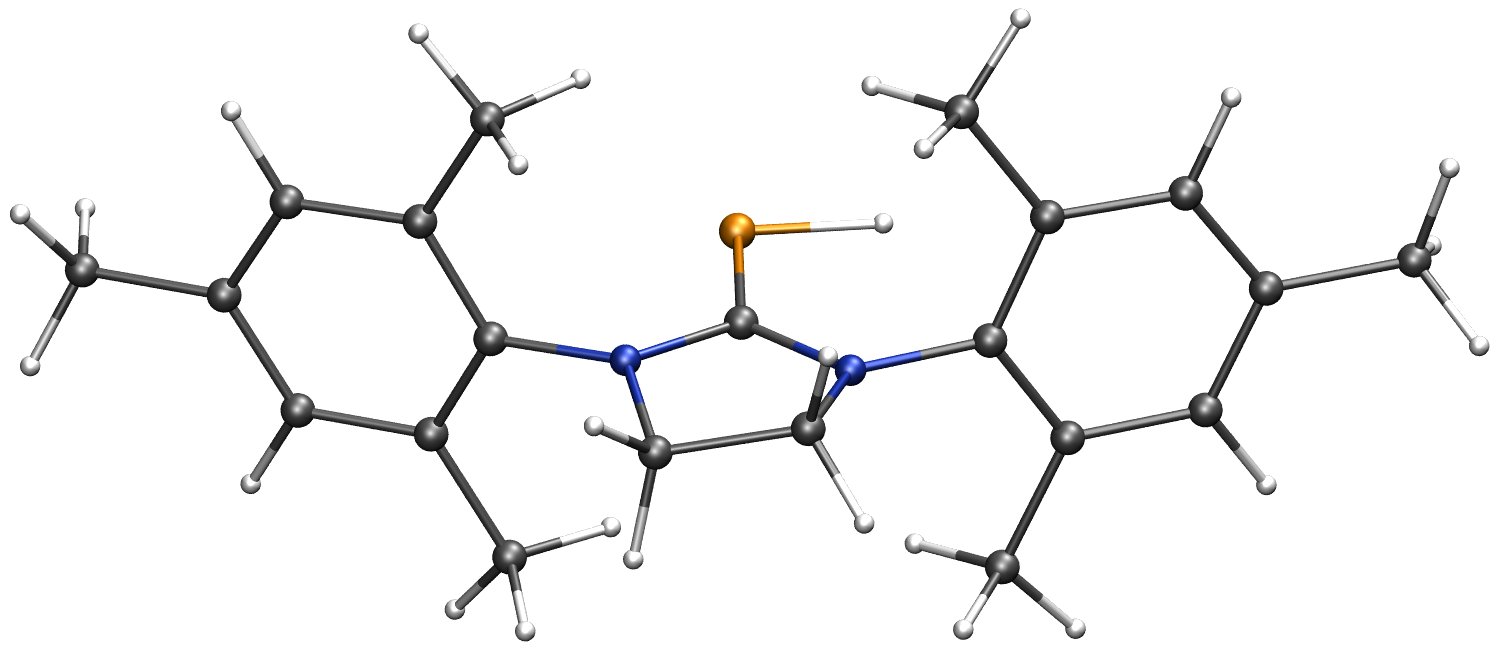
\includegraphics[width=0.6\textwidth]{1}
	\captionsetup{figurewithin = chapter}
	\captionsetup{font=small, labelfont=bf}\caption[Abbildung von SIMesPH]{Abbildung von SIMesPH, SIMes=1,3-bis(2,4,6-tri\-me\-thyl\-phe\-nyl)imi\-da\-zo\-lin-2-yli\-den (Kohlenstoff=grau, Wasserstoff=weiß, Stickstoff=blau und Phosphor=orange).}
\label{abb:cvh1}
\end{figure}

\begin{figure}[ht!]
	\centering
	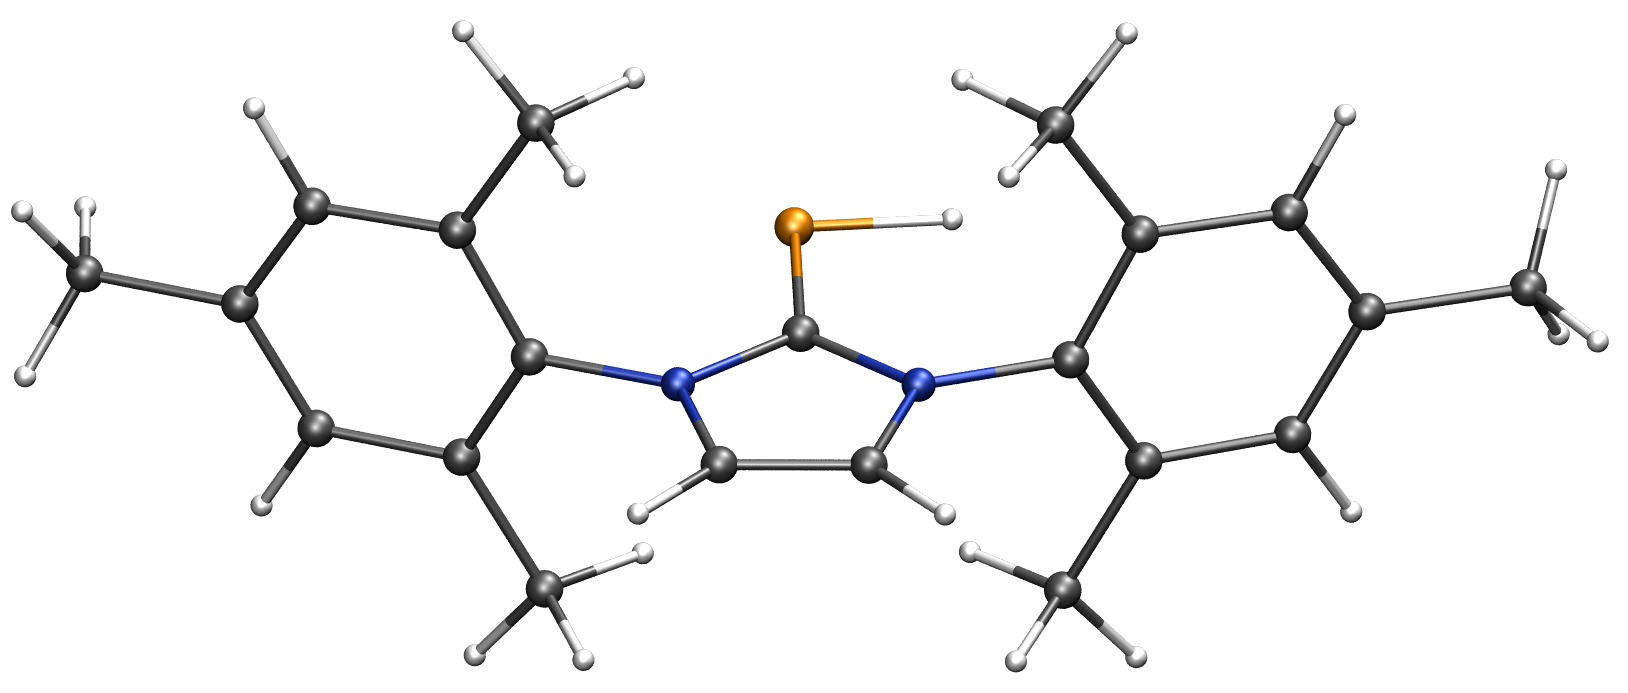
\includegraphics[width=0.6\textwidth]{2}
	\captionsetup{figurewithin = chapter}
	\captionsetup{font=small, labelfont=bf}\caption[Abbildung von IMesPH]{Abbildung von IMesPH, IMes=1,3-bis(2,4,6-tri\-me\-thyl\-phe\-nyl)imi\-da\-zol-2-yli\-den (Kohlenstoff=grau, Wasserstoff=weiß, Stickstoff=blau und Phosphor=orange).}
\label{abb:cvh2}
\end{figure}

\begin{figure}[ht!]
	\centering
	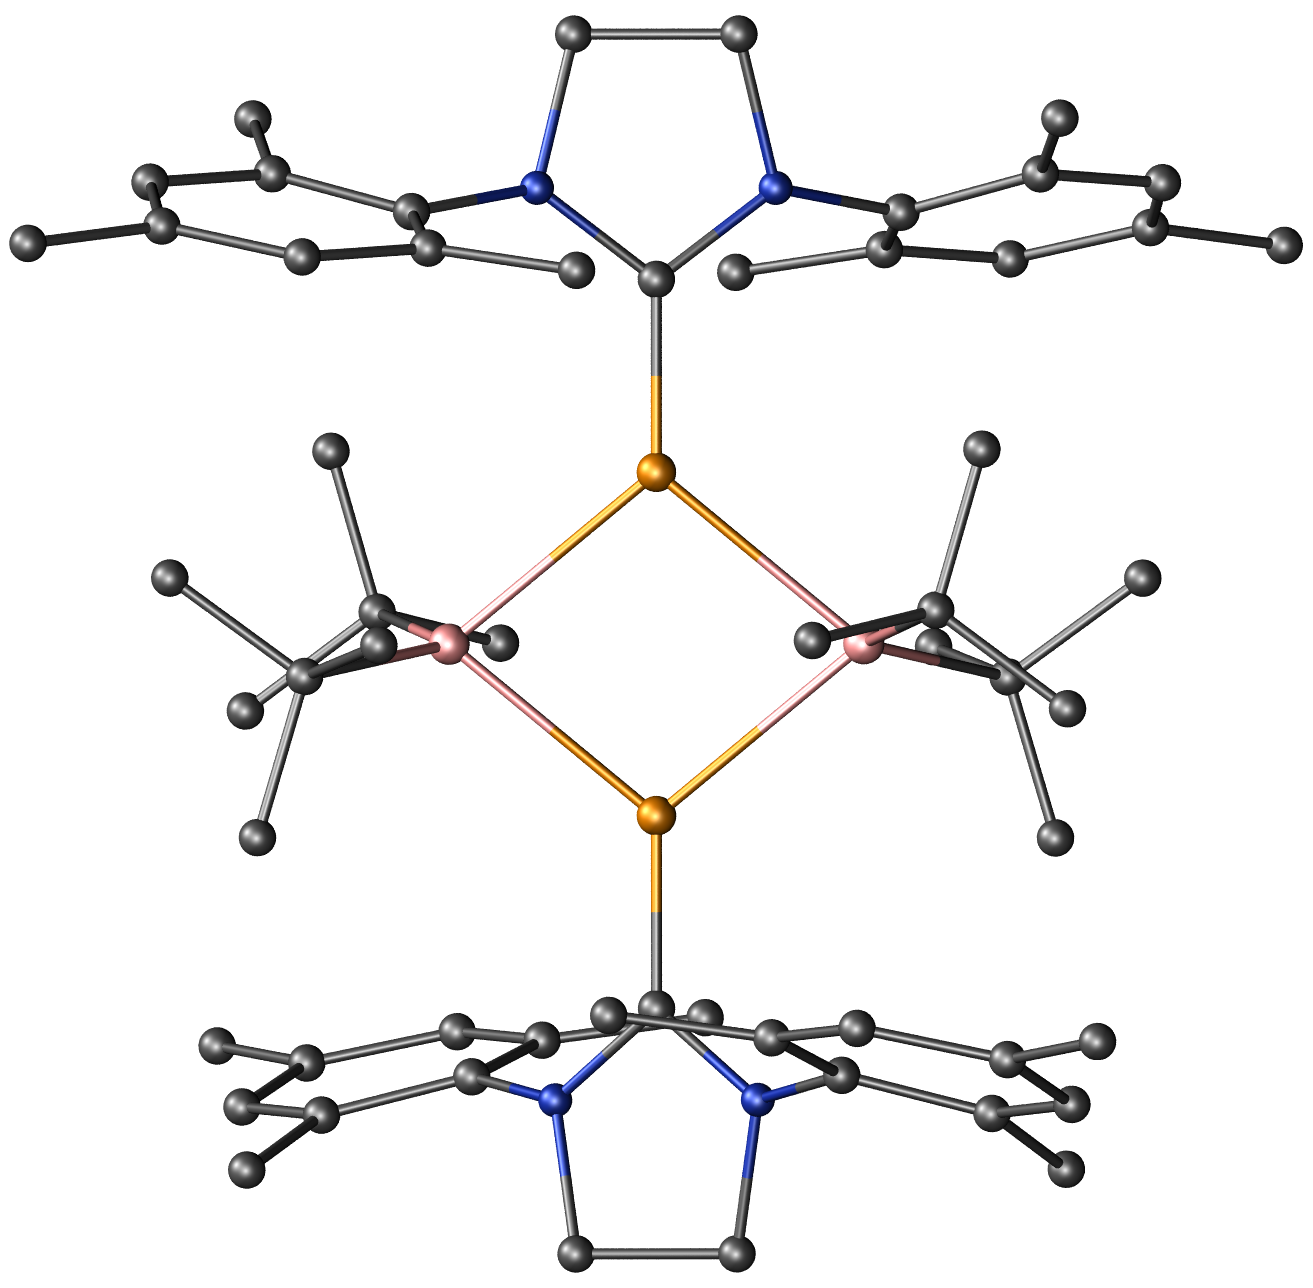
\includegraphics[width=0.6\textwidth]{3}
	\captionsetup{figurewithin = chapter}
	\captionsetup{font=small, labelfont=bf}\caption[{Abbildung von $[$SIMesPGa\textit{t}Bu$_2]_2$}]{Abbildung von $[$SIMesPGa\textit{t}Bu$_2]_2$, SIMes=1,3-bis(2,4,6-tri\-me\-thyl\-phe\-nyl)imi\-da\-zo\-lin-2-yli\-den (Kohlenstoff=grau, Stickstoff=blau, Phosphor=orange und Gallium=rosa). Die Wasserstoffatome wurden zur besseren Veranschaulichung bei der Abbildung weg gelassen.}
\label{abb:cvh3}
\end{figure}

\begin{figure}[ht!]
	\centering
	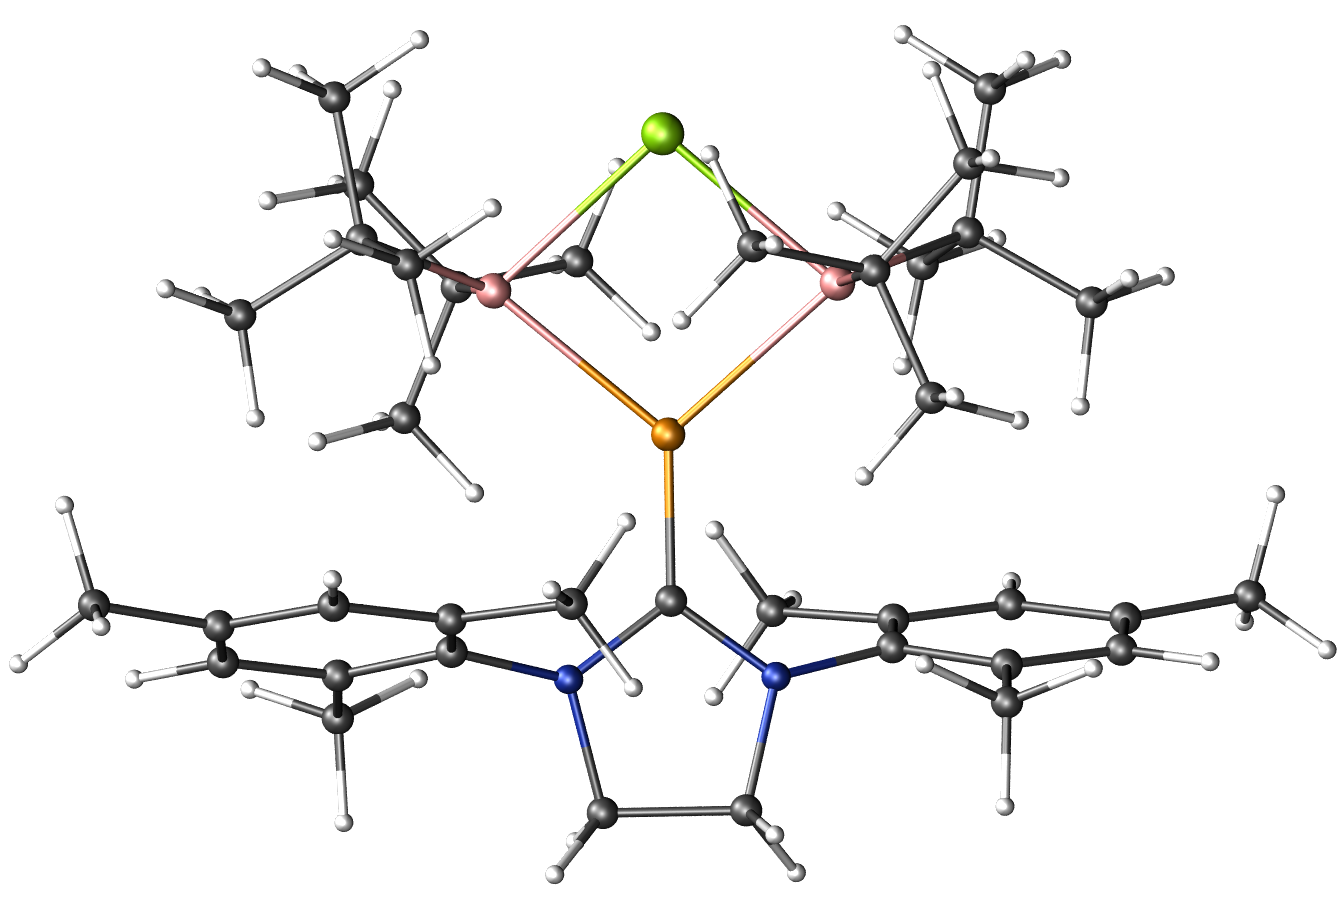
\includegraphics[width=0.6\textwidth]{4}
	\captionsetup{figurewithin = chapter}
	\captionsetup{font=small, labelfont=bf}\caption[Abbildung von SIMesP(Ga\textit{t}Bu$_2$)$_2$Cl]{Abbildung von SIMesP(Ga\textit{t}Bu$_2$)$_2$Cl, SIMes=1,3-bis(2,4,6-tri\-me\-thyl\-phe\-nyl)imi\-da\-zo\-lin-2-yli\-den (Kohlenstoff=grau, Wasserstoff=weiß, Stickstoff=blau, Phosphor=orange, Gallium=rosa und Chlor=grün).}
\label{abb:cvh4}
\end{figure}

\begin{figure}[ht!]
	\centering
	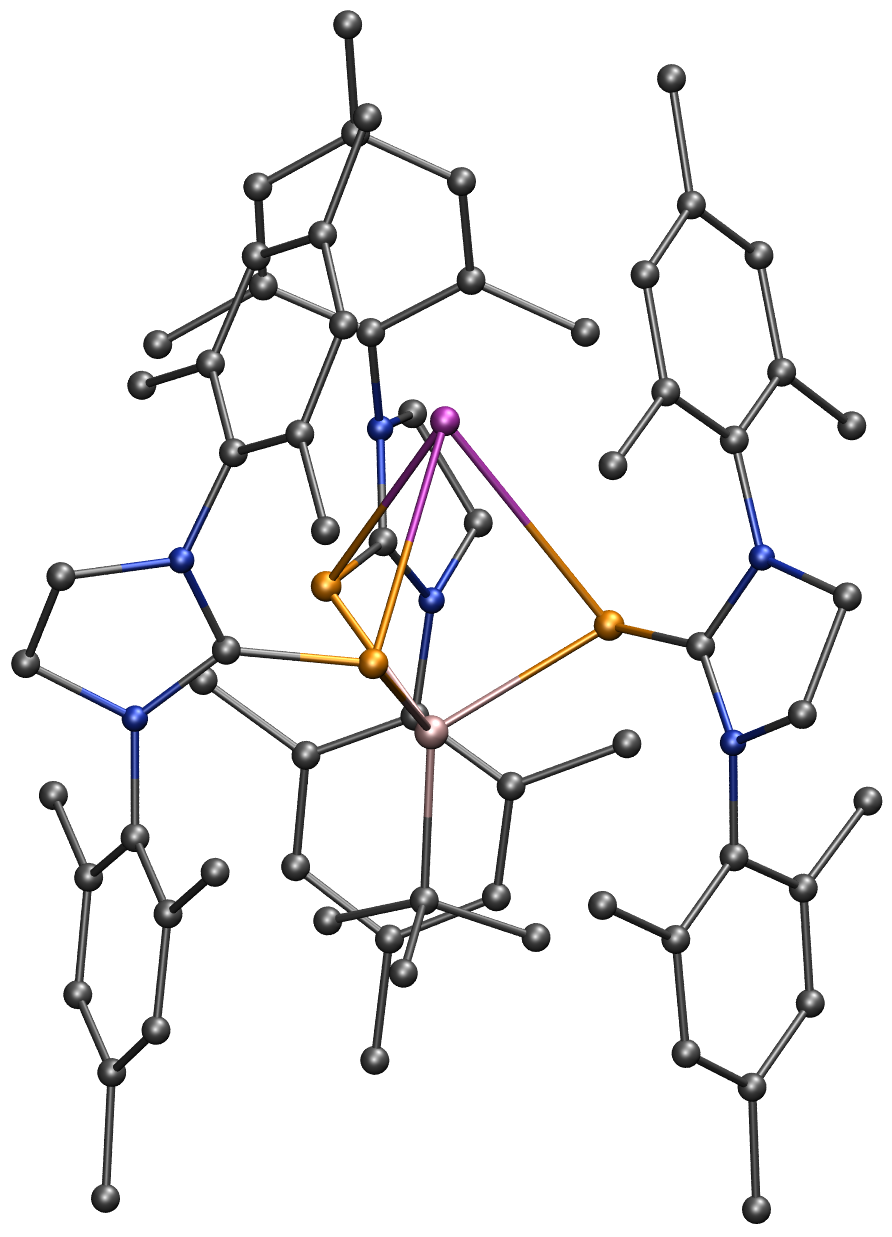
\includegraphics[width=0.5\textwidth]{5}
	\captionsetup{figurewithin = chapter}
	\captionsetup{font=small, labelfont=bf}\caption[Abbildung von K(SIMesP)$_3$Al\textit{t}Bu]{Abbildung von K(SIMesP)$_3$Al\textit{t}Bu, SIMes=1,3-bis(2,4,6-tri\-me\-thyl\-phe\-nyl)imi\-da\-zo\-lin-2-yli\-den (Kohlenstoff=grau, Stickstoff=blau, Phosphor=orange, Kalium=lila und Aluminium=hellrosa). Die Wasserstoffatome wurden zur besseren Veranschaulichung bei der Abbildung weg gelassen.}
\label{abb:cvh5}
\end{figure}

\begin{figure}[ht!]
	\centering
	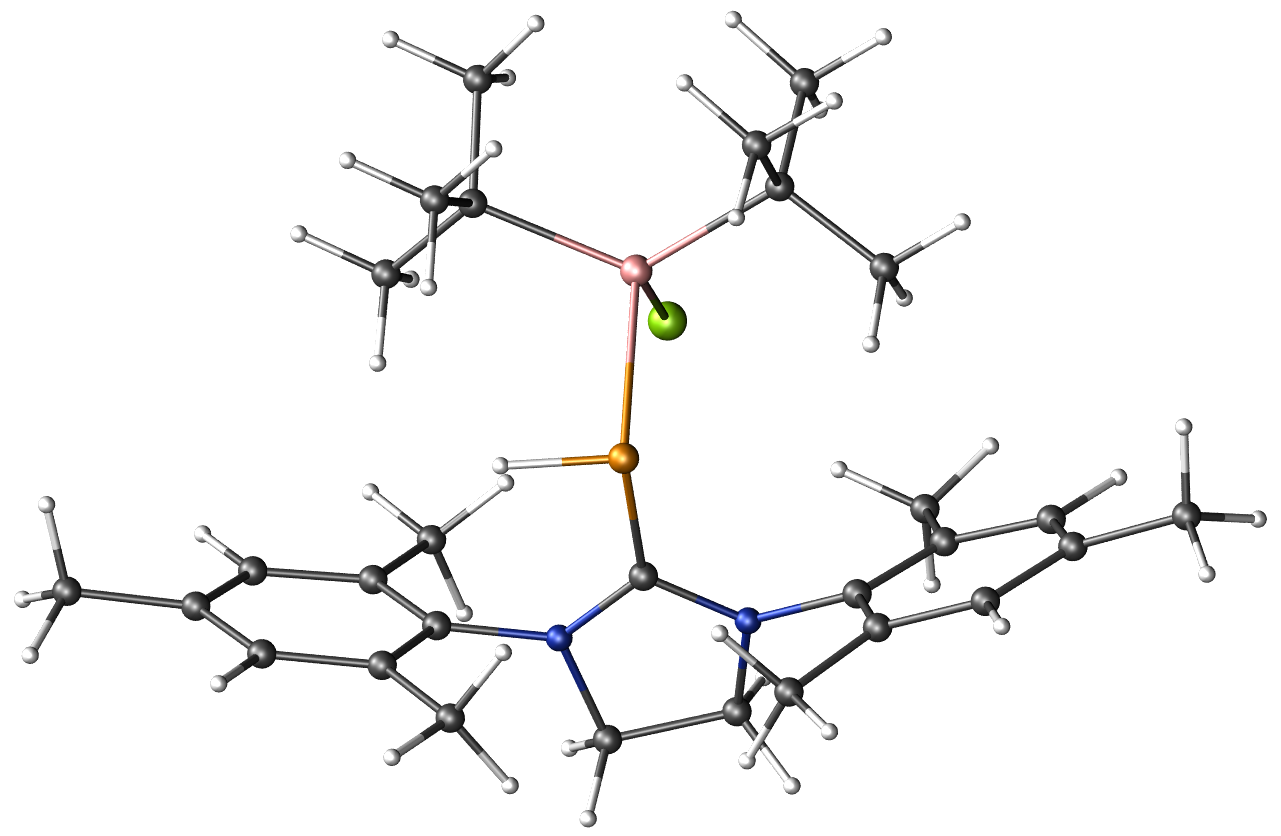
\includegraphics[width=0.6\textwidth]{6}
	\captionsetup{figurewithin = chapter}
	\captionsetup{font=small, labelfont=bf}\caption[Abbildung von SIMesPH\textit{t}Bu$_2$GaCl]{Abbildung von SIMesPH\textit{t}Bu$_2$GaCl, SIMes=1,3-bis(2,4,6-tri\-me\-thyl\-phe\-nyl)imi\-da\-zo\-lin-2-yli\-den (Kohlenstoff=grau, Wasserstoff=weiß, Stickstoff=blau, Phosphor=orange, Gallium=rosa und Chlor=grün).}
\label{abb:cvh6}
\end{figure}

\begin{figure}[ht!]
	\centering
	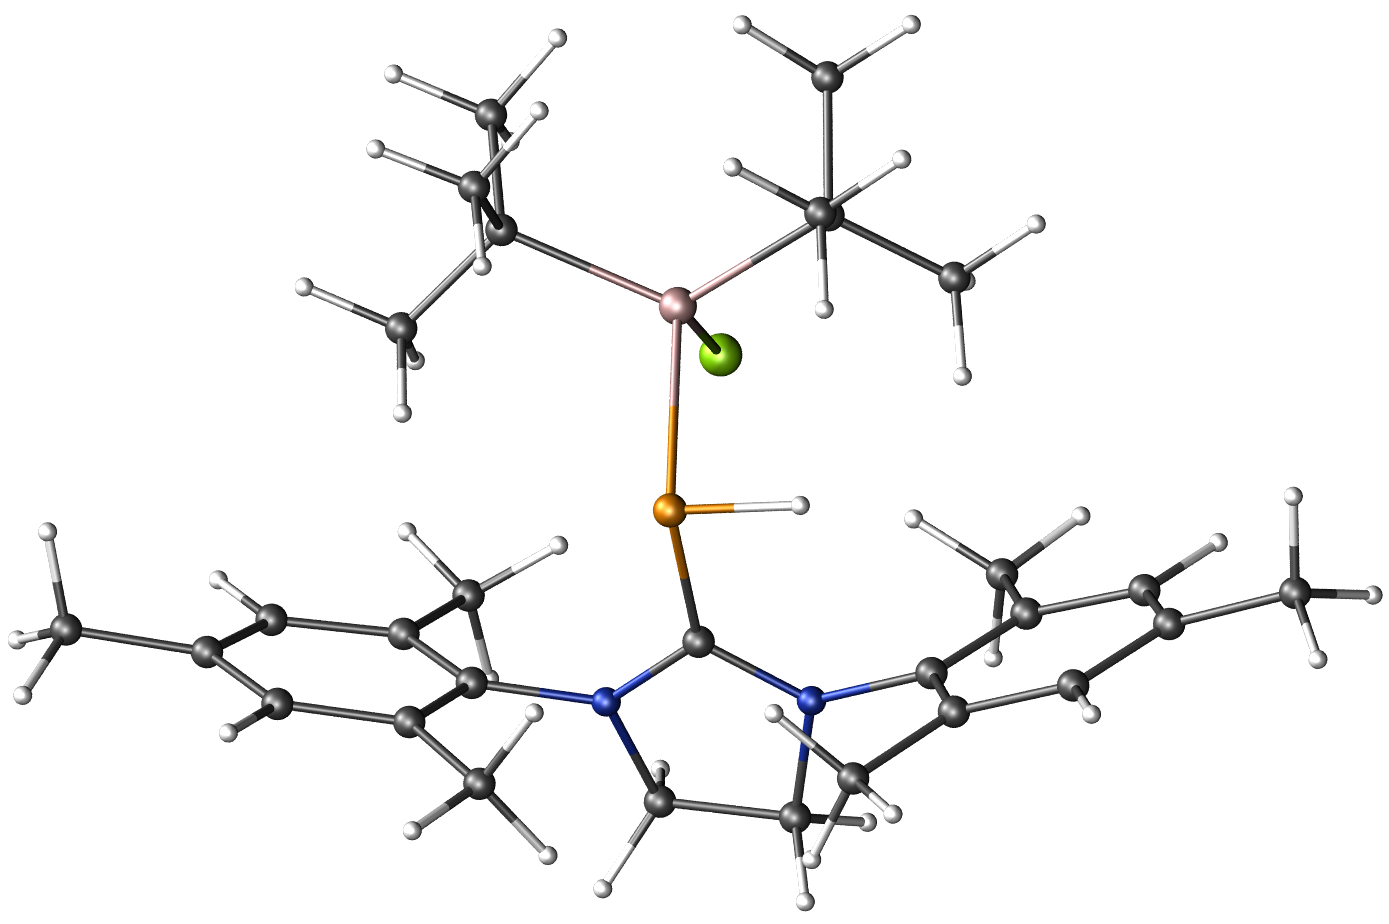
\includegraphics[width=0.6\textwidth]{7}
	\captionsetup{figurewithin = chapter}
	\captionsetup{font=small, labelfont=bf}\caption[Abbildung von SIMesPH\textit{t}Bu$_2$AlCl]{Abbildung von SIMesPH\textit{t}Bu$_2$AlCl, SIMes=1,3-bis(2,4,6-tri\-me\-thyl\-phe\-nyl)imi\-da\-zo\-lin-2-yli\-den (Kohlenstoff=grau, Wasserstoff=weiß, Stickstoff=blau, Phosphor=orange, Aluminium=hellrosa und Chlor=grün).}
\label{abb:cvh7}
\end{figure}


\FloatBarrier
\newpage

\subsection{\texorpdfstring{$[$Hg$_8$Te$_8$(Te$_2$)$_4$]$^{8-}$}{[Hg\_8Te\_8(Te\_2)\_4]8-}: Ein anorganisches Porphyrin?}
Die Implementierung des \ac{cosmo}\supercite{klamt1993cosmo} und der \acp{ecp} in das \texttt{mpshift} Modul lieferte die notwendigen Voraussetzungen, um einen tieferen Einblick über magnetische Eigenschaften in anionischen Verbindungen, welche schwere Elemente beinhalten, zu erhalten. Ein Beispiel dafür ist das in der Gruppe von Stephanie Dehnen synthetisierte $[$Hg$_8$Te$_8$(Te$_2$)$_4$]$^{8-}$\supercite{dehnenhg4te8}, welches auf der linken Seite in Abbildung \ref{abb:hg8te16undb8s16} gezeigt ist. Die Seitenansicht zeigt das Molekül mit TPSSh\supercite{tao2003climbing}/def2-TZVP\supercite{weigend2005balanced} optimierten Strukturparametern. Zusätzlich wurden die entsprechenden Auxiliarbasisfunktionen\supercite{weigend2006accurate} und \acp{ecp}\supercite{peterson2003systematically} verwendet. Die Kompensation der Ladung erfolgte durch das \ac{cosmo}. In der Abbildung ist zu erkennen, dass das Anion nicht vollständig planar ist und damit auch leicht von der idealen $D_{4\textrm{h}}$ symmetrischen Struktur abweicht. 
\begin{figure}[ht!]
	\centering
	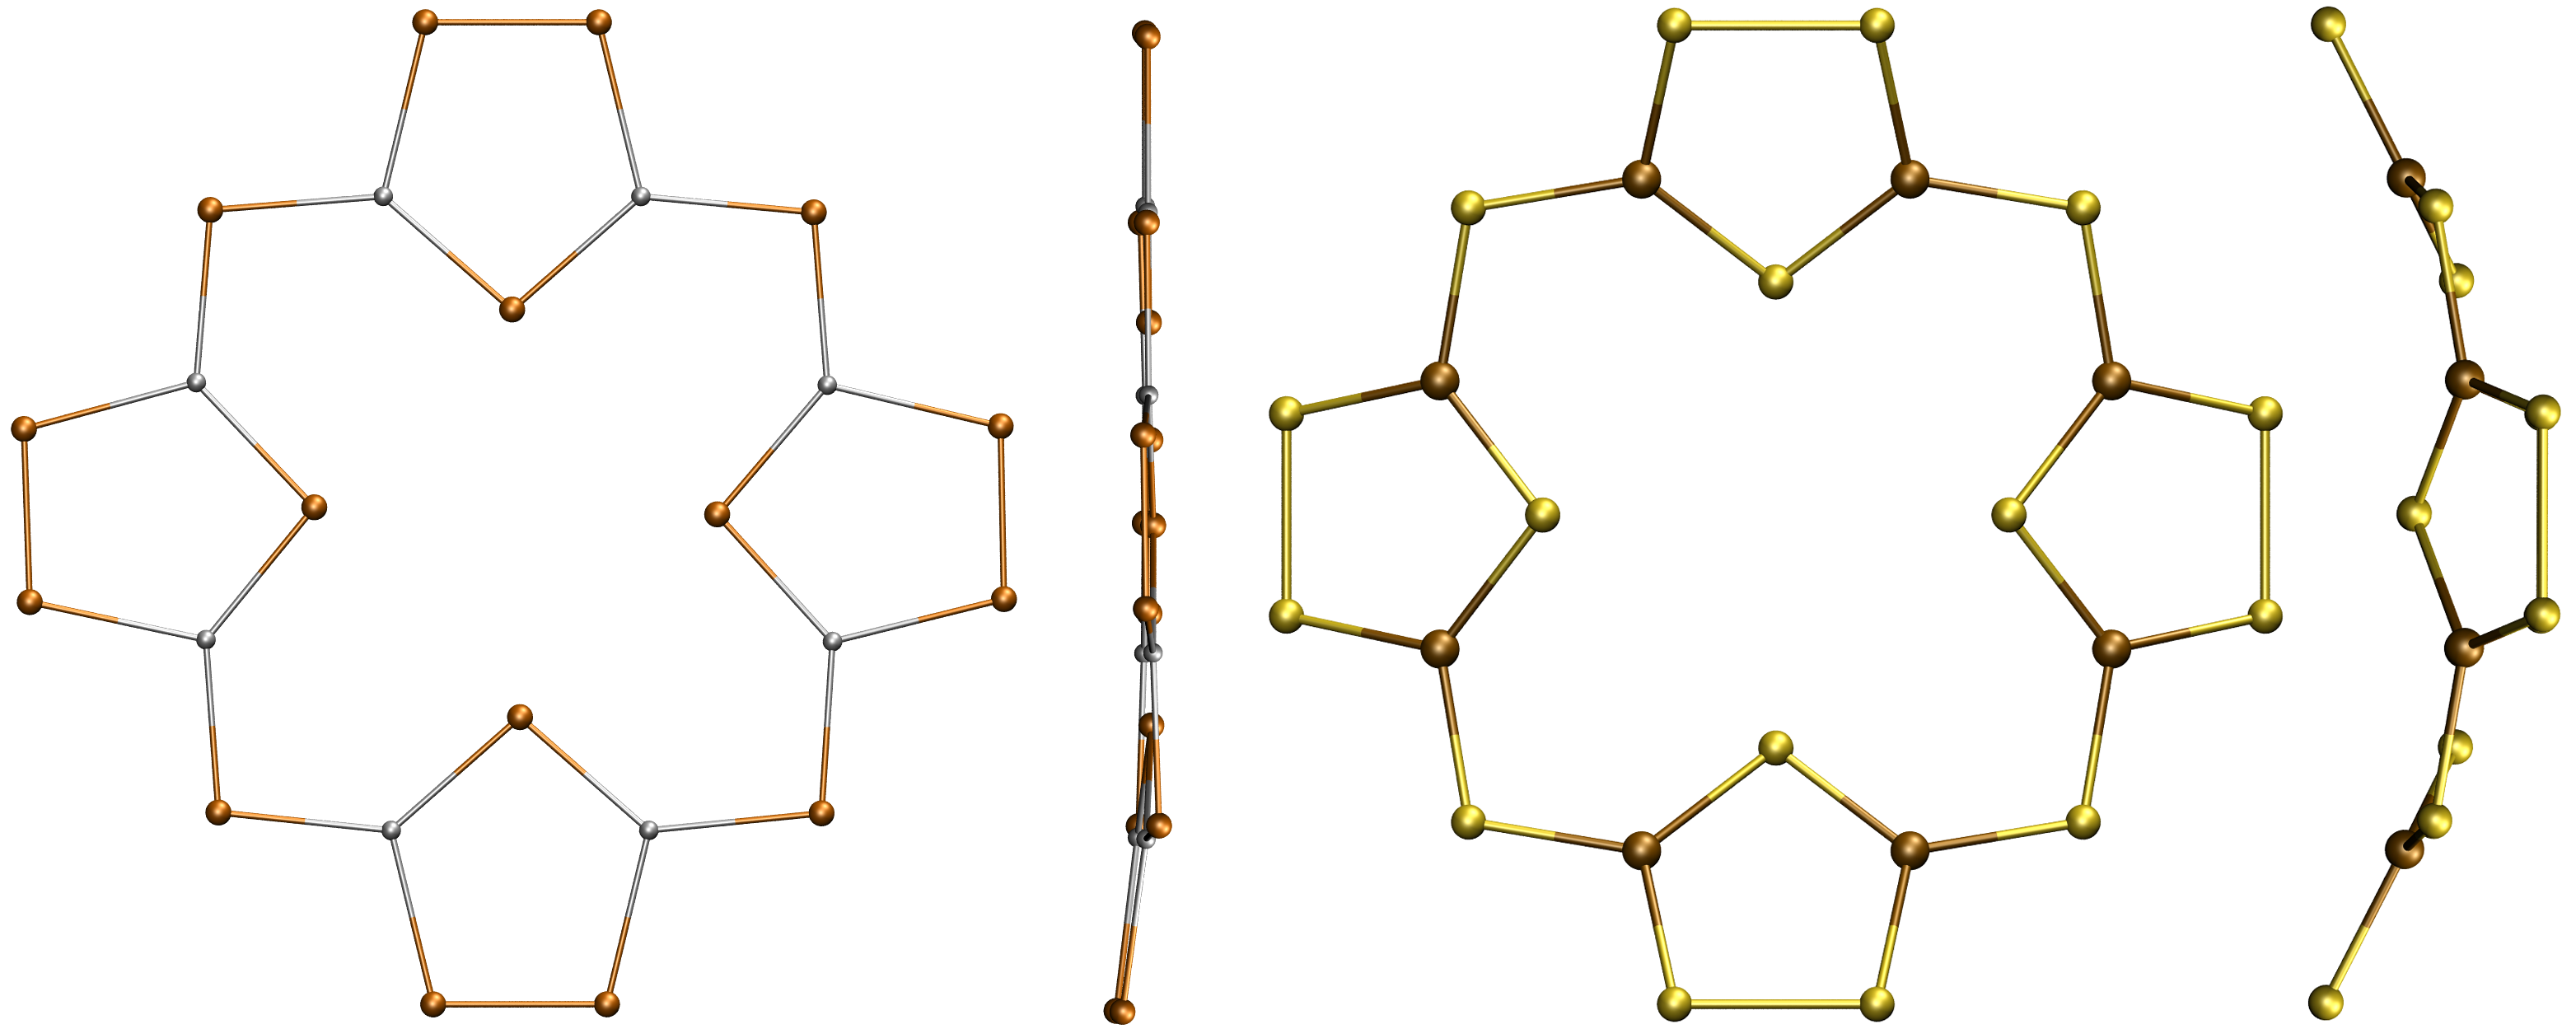
\includegraphics[width=1.0\textwidth]{hg8te16undb8s16}
	\captionsetup{figurewithin = chapter}
	\captionsetup{font=small, labelfont=bf}\caption[{Abbildung von $[$Hg$_8$Te$_{16}]^{8-}$ und B$_8$S$_{16}$}]{{Draufsicht und Seitenansicht von $[$Hg$_8$Te$_{16}]^{8-}$} (links) und B$_8$S$_{16}$ (rechts)(Quecksilber=silber, Tellur=orangebraun, Bohr=braun und Schwefel=gelb).}
\label{abb:hg8te16undb8s16}
\end{figure}
%\begin{figure}[ht!]
%	\centering
%	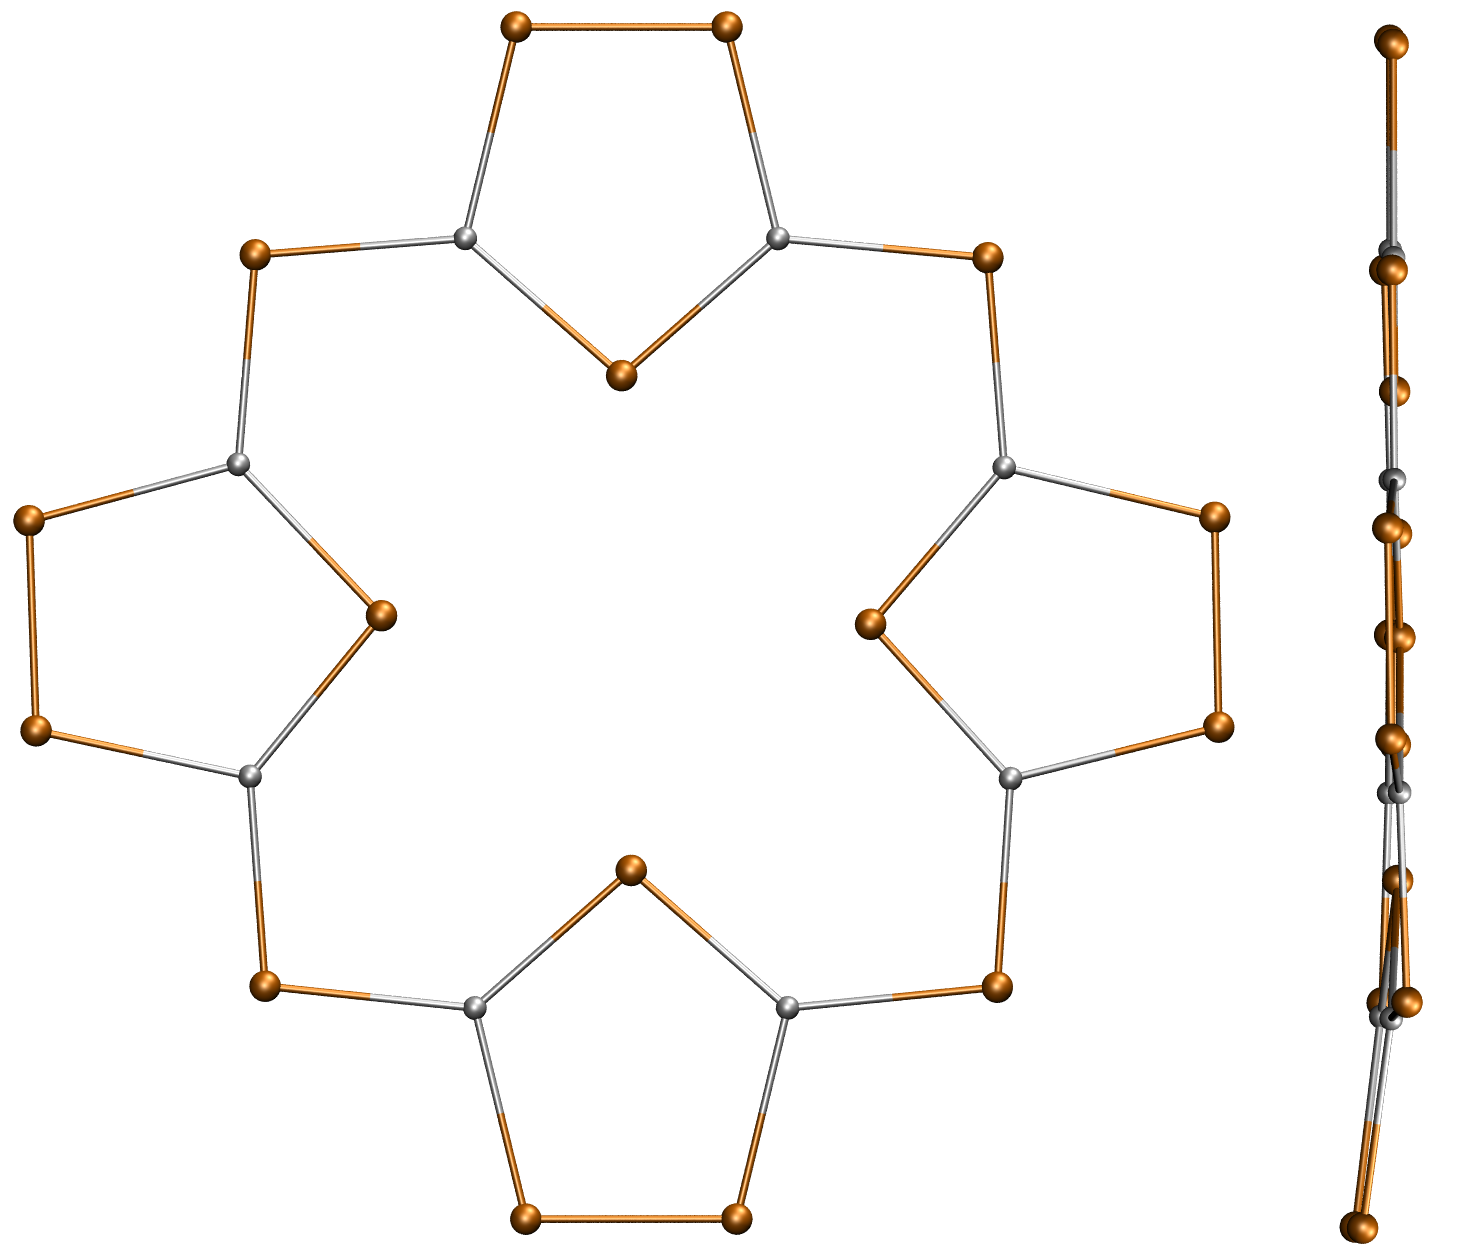
\includegraphics[width=0.6\textwidth]{hg8te16}
%	\captionsetup{figurewithin = chapter}
%	\captionsetup{font=small, labelfont=bf}\caption[{Abbildung von $[$Hg$_8$Te$_{16}]^{8-}$}]{{Abbildung von $[$Hg$_8$Te$_{16}]^{8-}$}(Quecksilber=silber, Tellur=orangebraun). Draufsicht links und Seitenansicht rechts.}
%\label{abb:hg8te16}
%\end{figure}

Zusätzlich wurde ebenfalls das bereits bekannte B$_8$S$_{16}$\supercite{krebs1980b8s16} (Abbildung \ref{abb:hg8te16undb8s16} rechts) untersucht. Hier ist die Abweichung des Moleküls mit optimierten Strukturparametern von der planaren Struktur noch deutlich größer, wie die Seitenansicht deutlich zeigt. Die $D_{4\textrm{h}}$ symmetrische Struktur weißt eine schwache imaginäre Mode von etwa -10 Wellenzahlen auf welche genau der Gerüstschwingung entspricht, welche das Durchschwingen des Moleküls beschreibt. Ebenfalls bekannt ist das schwerere Homolog B$_8$Se$_{16}$.
%\begin{figure}[ht!]
%	\centering
%	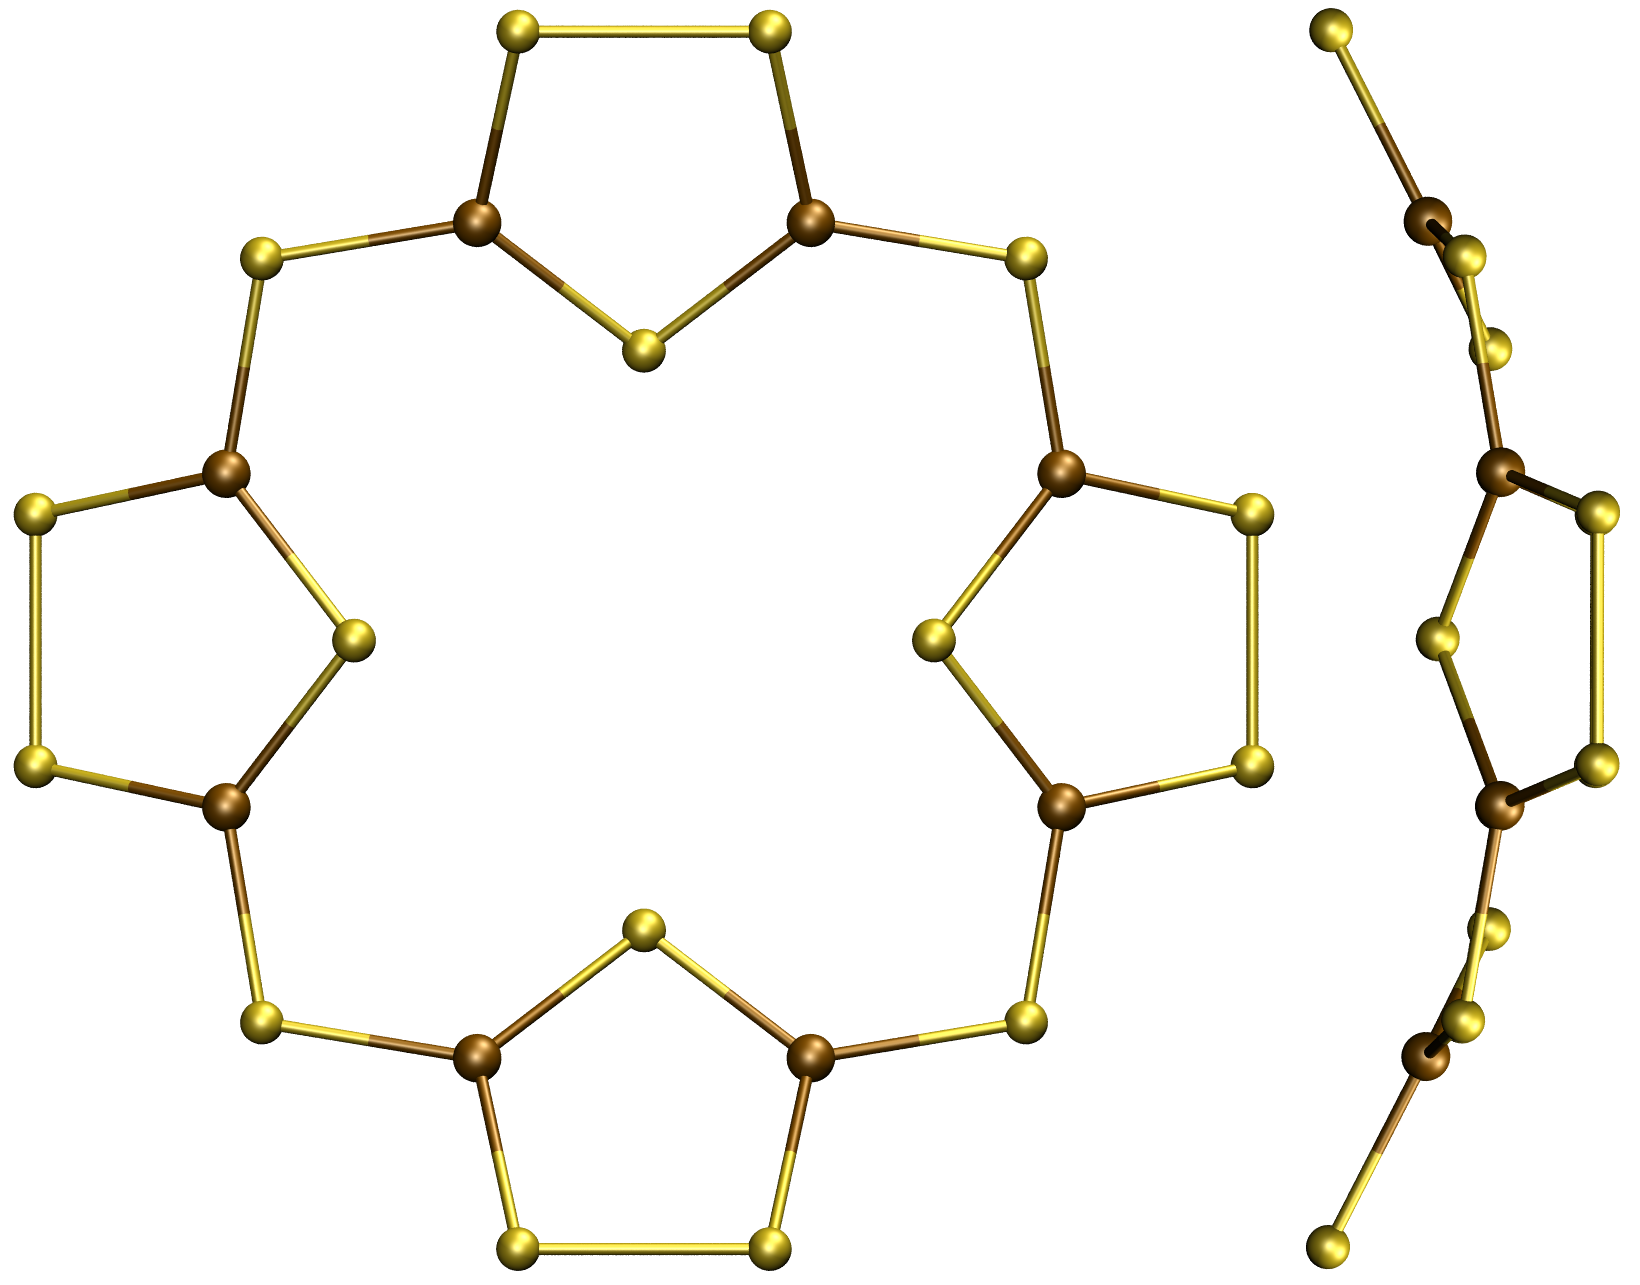
\includegraphics[width=0.6\textwidth]{b8s16}
%	\captionsetup{figurewithin = chapter}
%	\captionsetup{font=small, labelfont=bf}\caption[Abbildung von B$_8$S$_{16}$]{Abbildung von B$_8$S$_{16}$(Bohr=braun, Schwefel=gelb). Draufsicht links und Seitenansicht rechts.}
%\label{abb:b8s16}
%\end{figure}

Aufgrund ihrer strukturellen Ähnlichkeit mit dem organischen Porphyrin liegt es nahe, den aromatischen Charakter der Verbindungen zu untersuchen. Als Maß für die Aromatizität einer Verbindung kann der durch einen definierten Ring fließende Elektronenstrom - kurz Ringstrom - angesehen werden. Je diatropischer der Gesamtstrom (d.h. der Strom fließt im Uhrzeigersinn), desto aromatischer ist die Verbindung. Ein stark paratropischer Strom (Strom entgegen des Uhrzeigersinns) deutet dabei auf eine antiaromatische Verbindung hin. Sind die diatropischen und paratropischen Beiträge in etwa von der selben Größe, dann verschwindet der Gesamtstrom - die Verbindung ist nichtaromatisch. Bei der Berechnung der Ringströme mit \ac{gimic} wird dabei so vorgegangen, dass der Strom der durch eine senkrecht zur Bindungsachse stehenden Ebene fließt, integriert wird. In den oben erwähnten Beispielen kann weiterhin zwischen einem lokalen Ringstrom in den vier Fünfringen und einem globalen Ringstrom um das gesamte Molekül unterschieden werden. Bei den Berechnungen stellte sich heraus, dass alle drei Verbindungen, $[$Hg$_8$Te$_{16}]^{8-}$, B$_8$S$_{16}$ und B$_8$Se$_{16}$ einen schwachen lokalen Ringstrom in den pyrrolartigen fünfgliedrigen Ringen aufweisen. Diese betragen \unit[5.8]{nA/T} in $[$Hg$_8$Te$_{16}]^{8-}$ \unit[3.25]{nA/T} in B$_8$S$_{16}$ und \unit[3.28]{nA/T} in B$_8$Se$_{16}$. Im Vergleich dazu beträgt der Ringstrom in einem Benzolmolekül etwa \unit[12]{nA/T}\supercite{fliegl2012aromatic}. Die globalen Ringströme in den drei Verbindungen sind mit \unit[0.24]{nA/T}, \unit[0.81]{nA/T} und \unit[0.79]{nA/T} verschwindend gering. Im Vergleich dazu liegt der globale Ringstrom des organischen Porphyrins bei etwa \unit[27]{nA/T}. Dieser spaltet sich in den fünfgliedrigen Ringen in einen äußeren und inneren Pfad auf, welche jeweils einen Ringstrom von etwa \unit[13]{nA/T} aufweisen. Der lokale Ringstrom in den fünfgliedrigen Ringen ist schwächer als \unit[1]{nA/T}.\supercite{fliegl2012aromatic} In sogenannten \ac{lic} Plots lassen sich die Ringströme in einer gewählten Ebene visualisieren. Dies wurde für das organische Porphyrin und die drei Verbindungen $[$Hg$_8$Te$_{16}]^{8-}$, B$_8$S$_{16}$ und B$_8$Se$_{16}$ gemacht und die entsprechenden Plots sind in der Abbildung \ref{abb:lic} zu sehen. Beim Porphyrin ist eindeutig der globale Ringstrom zu erkennen, welcher sich in den fünfgliedrigen Ringen in zwei Pfade aufspaltet. im Vergleich dazu weisen die anderen Verbindungen lediglich schwache lokale Ströme in den fünfgliedrigen Ringen auf.
Diese Befunde lassen sich dadurch erklären, dass im Porphyrin eine völlig andere elektronische Situation vorliegt. Die Aromatizität und die damit verbundenen Ringströme basieren auf einem delokalisierten $\pi$-System. Beispielsweise lassen sich im $[$Hg$_8$Te$_{16}]^{8-}$ alle \acp{mo} durch Anwenden einer Lokalisierungsprozedur\supercite{boys1960sf} zu Zweizentren-Zweielektronen-Bindungen und freien Elektronenpaaren lokalisieren. Dabei werden s-artige Einfachbindungen zwischen den benachbarten Atomen und zwei freie Elektronenpaare pro Telluratom erhalten. 

 

\begin{figure}[ht!]
	\centering
	\includegraphics[width=1.0\textwidth]{1bohr}
	\captionsetup{figurewithin = chapter}
	\captionsetup{font=small, labelfont=bf}\caption[{Ringströme in Porphyrin, $[$Hg$_8$Te$_{16}]^{8-}$, B$_8$S$_{16}$ und B$_8$Se$_{16}$}]{Ringströme in Porphyrin (oben links), $[$Hg$_8$Te$_{16}]^{8-}$ (oben rechts), B$_8$S$_{16}$ (unten links) und B$_8$Se$_{16}$ (unten rechts) \unit[1]{bohr} oberhalb der Molekülebene, dargestellt zwischen \unit[0]{a.u.} (blau) und \unit[0.07]{a.u.}.}
\label{abb:lic}
\end{figure}

\FloatBarrier
Das fehlende $\pi$-System im $[$Hg$_8$Te$_{16}]^{8-}$ sorgt für eine gewisse strukturelle Flexibilität des Makrozyklus. Dadurch können unterschiedliche Koordinationspolyeder und Koordinationszahlen realisiert werden. Die Strukturparameter wurden exemplarisch für der Komplexierung der Metallkationen Zn$^{2+}$, Cu$^+$ , Ce$^{4+}$ und Ti$^{4+}$ optimiert und die erhaltenen Strukturen sind in Abbildung \ref{abb:komplexierung} gezeigt. Für Zn$^{2+}$ und Cu$^+$ ist zu erkennen, dass es dabei im Wesentlichen zu einer Verzerrung des Makrozyklus kommt um eine tetraedrische Koordination zu ermöglichen. Im Falle der Ce$^{4+}$ und Ti$^{4+}$ Kationen führt die Komplexierung zu einer deutlich ausgeprägteren Umordnung der Atome. Damit lässt sich sowohl die bevorzugt größere Koordinationszahl des Ce$^{4+}$ als auch die Anpassung an den deutlich geringeren Ionenradius des Ti$^{4+}$ realisieren.

\begin{figure}[ht!]
	\centering
	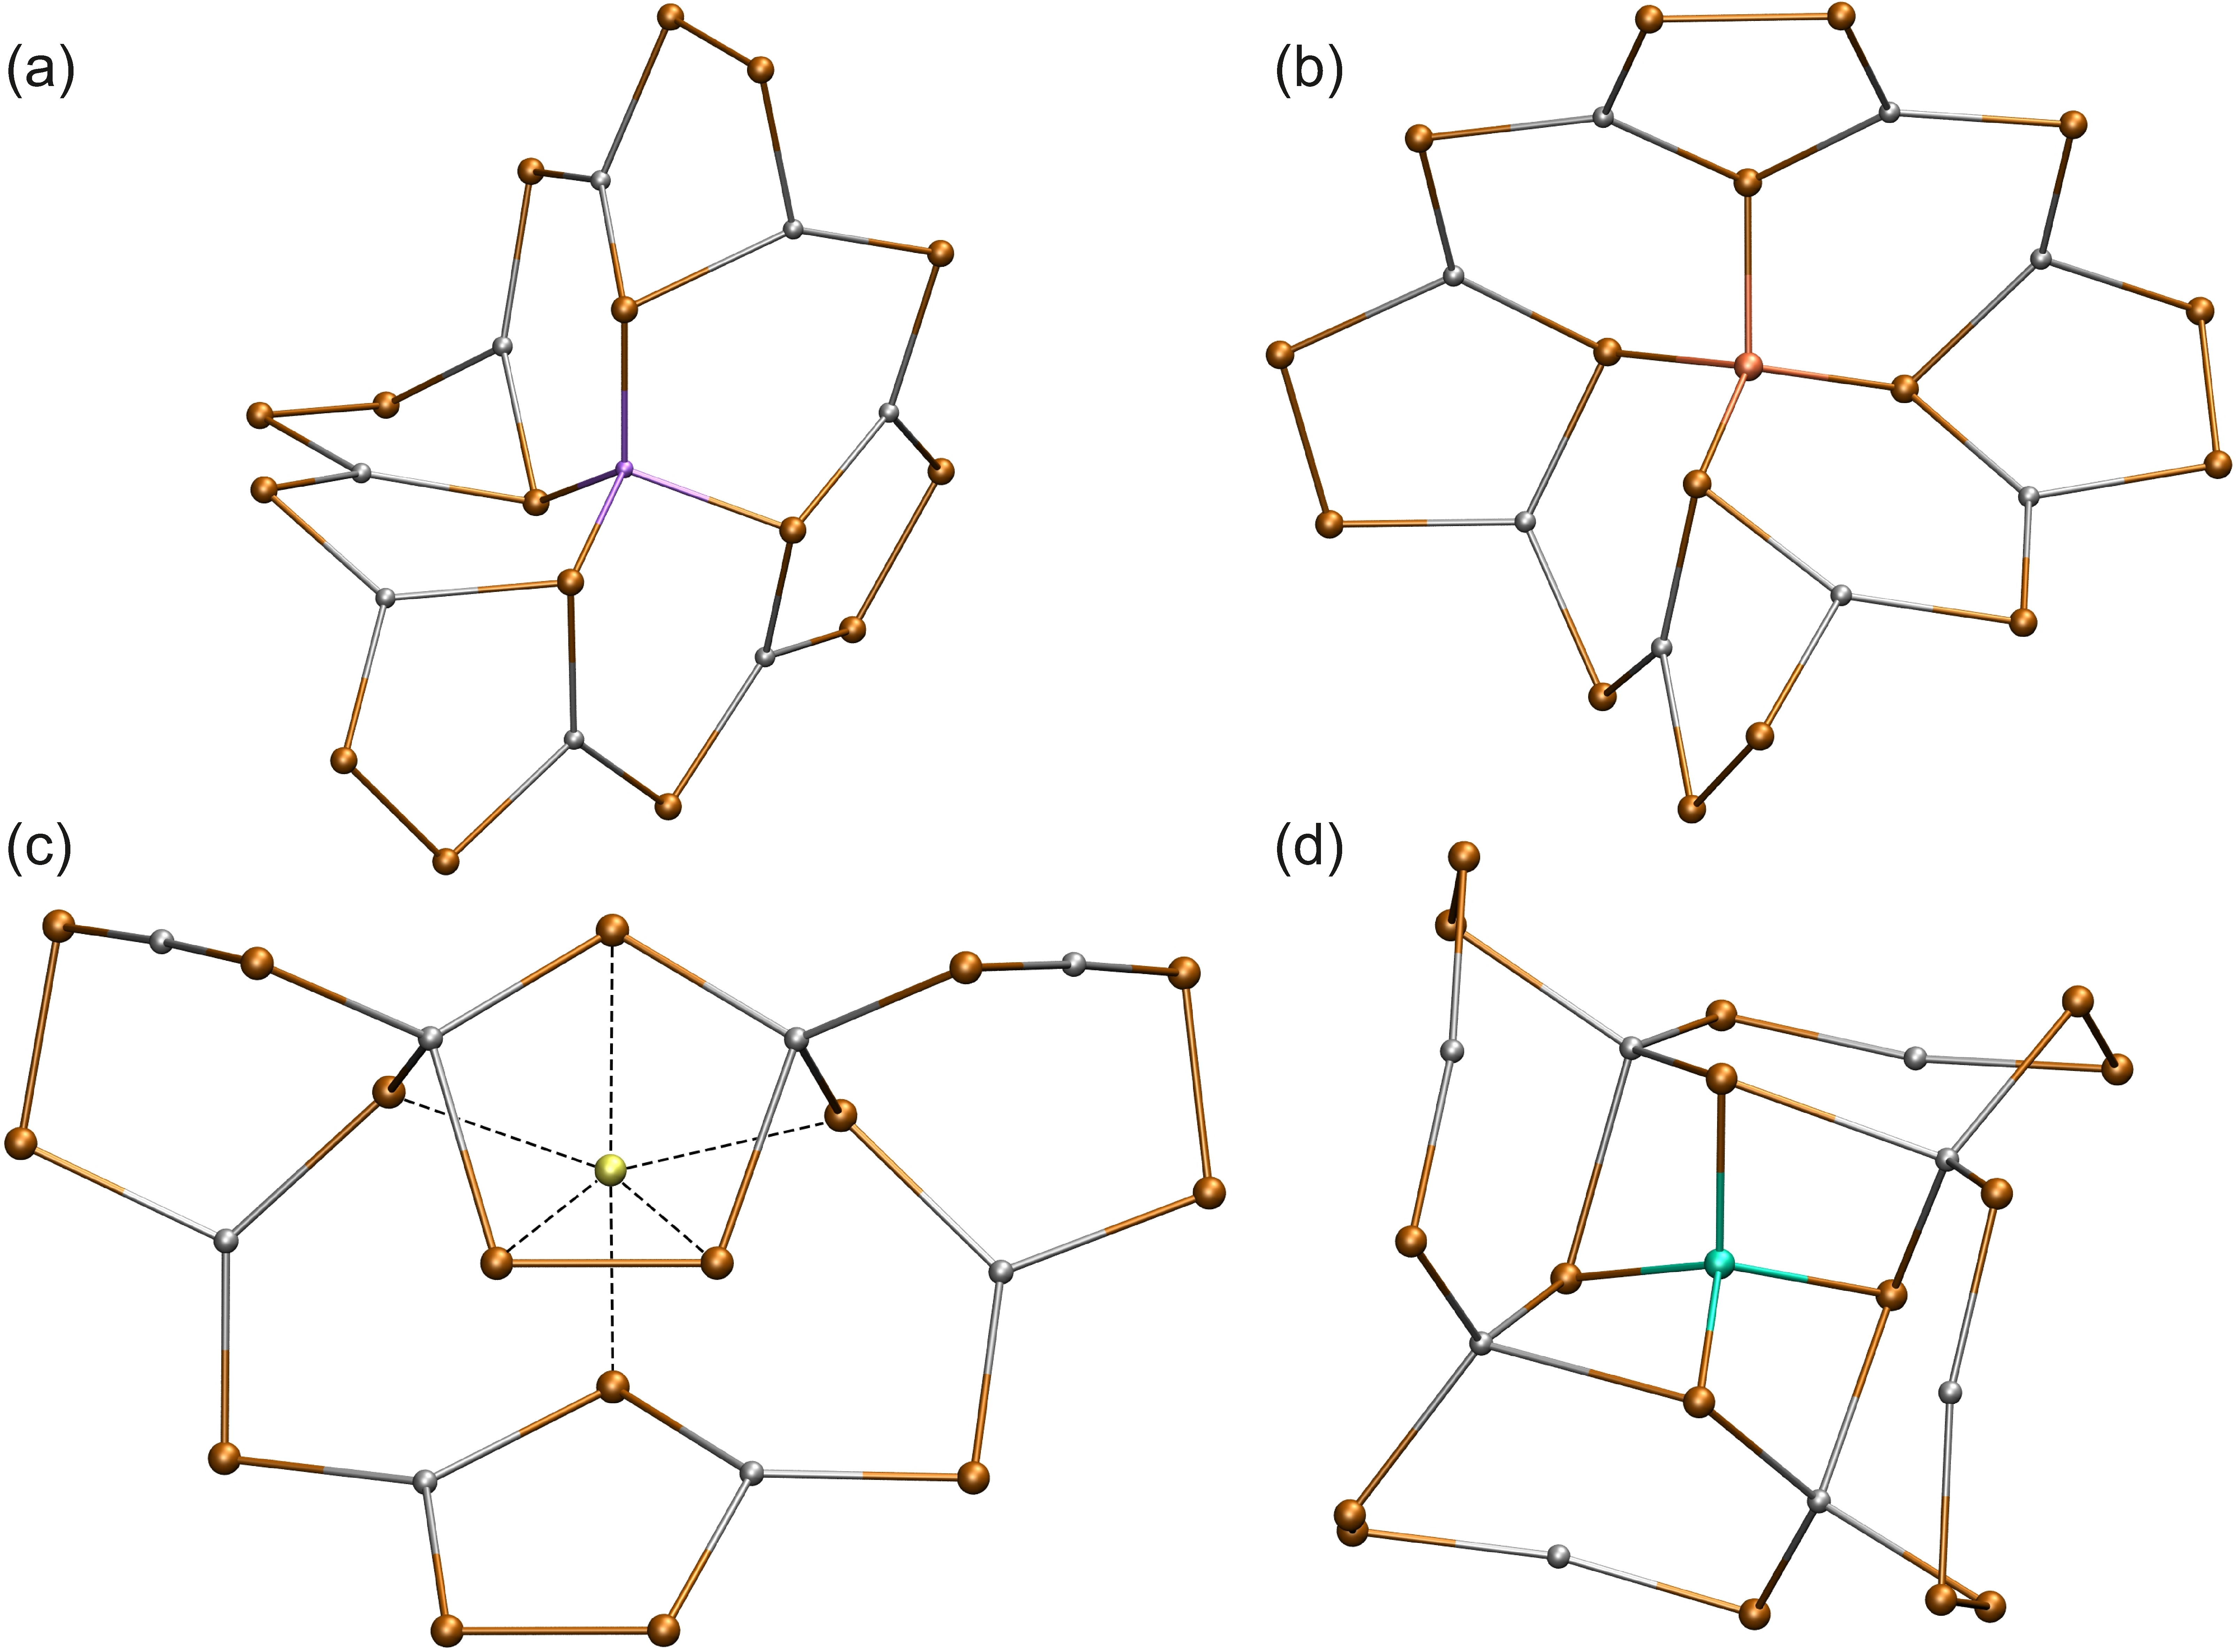
\includegraphics[width=1.0\textwidth]{komplexierung}
	\captionsetup{figurewithin = chapter}
	\captionsetup{font=small, labelfont=bf}\caption[{Abbildungen der hypothetischen Komplexe [M@Hg$_8$Te$_{16}]^{(8-q)-}$ (M$^{q+}$ = Zn$^{2+}$, Cu$^+$ , Ce$^{4+}$ und Ti$^{4+}$)}]{{Abbildung der hypothetischen Komplexe [M@Hg$_8$Te$_{16}]^{(8-q)-}$ (M$^{q+}$ = Zn$^{2+}$ (oben links), Cu$^+$ (oben rechts), Ce$^{4+}$ (unten links) und Ti$^{4+}$ (unten rechts))} zur Veranschaulichung der strukturellen Flexibilität von $[$Hg$_8$Te$_{16}]^{8-}$ (Quecksilber=silber, Tellur=orangebraun, Zink=lilablau, Kupfer=kupfer, Cer=hellgelb, Titan=türkis). }
\label{abb:komplexierung}
\end{figure}

%\begin{figure}[ht!]
%	\centering
%	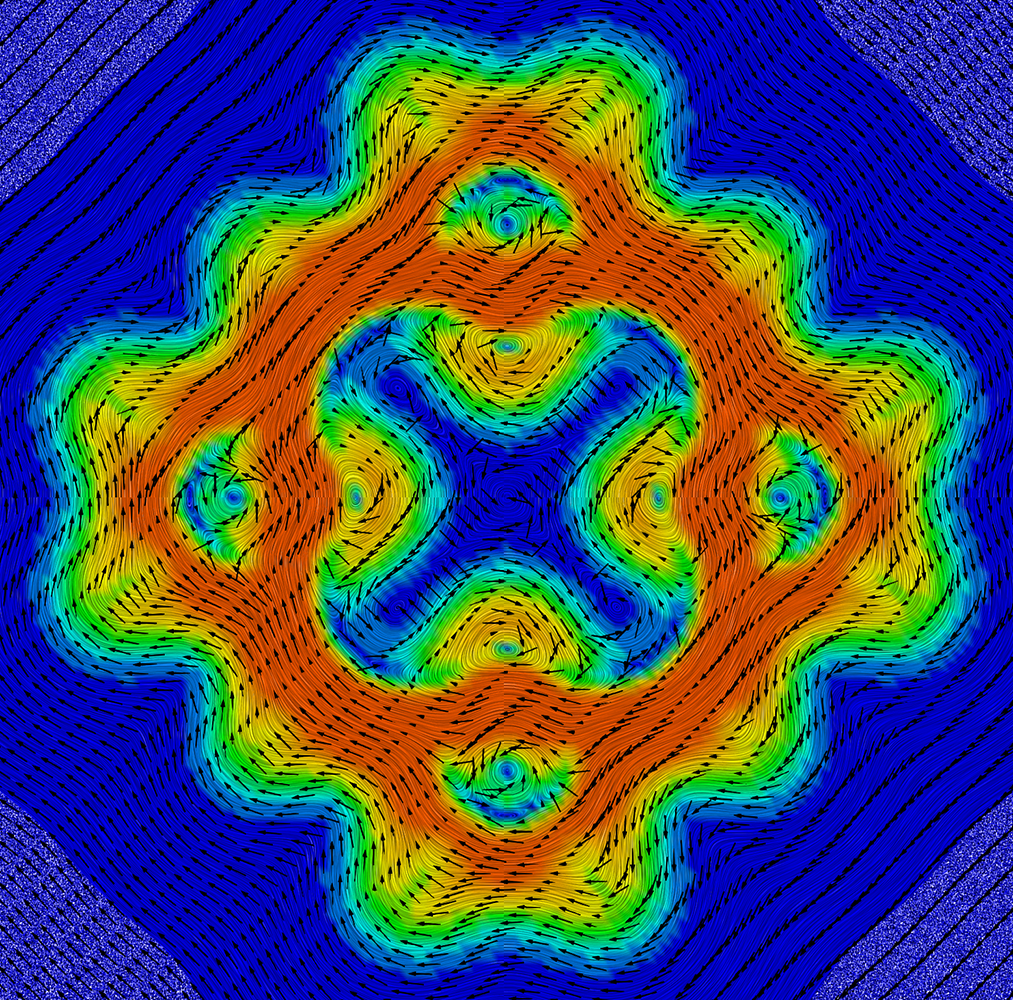
\includegraphics[width=0.6\textwidth]{porph_1bohr}
%	\captionsetup{figurewithin = chapter}
%	\captionsetup{font=small, labelfont=bf}\caption[Ringströme in Porphyrin]{Ringströme in Porphyrin \unit[1]{bohr} oberhalb der Molekülebene, dargestellt zwischen \unit[0]{a.u.} (blau) und \unit[0.07]{a.u.}.}
%\label{abb:porphlic}
%\end{figure}
%
%\begin{figure}[ht!]
%	\centering
%	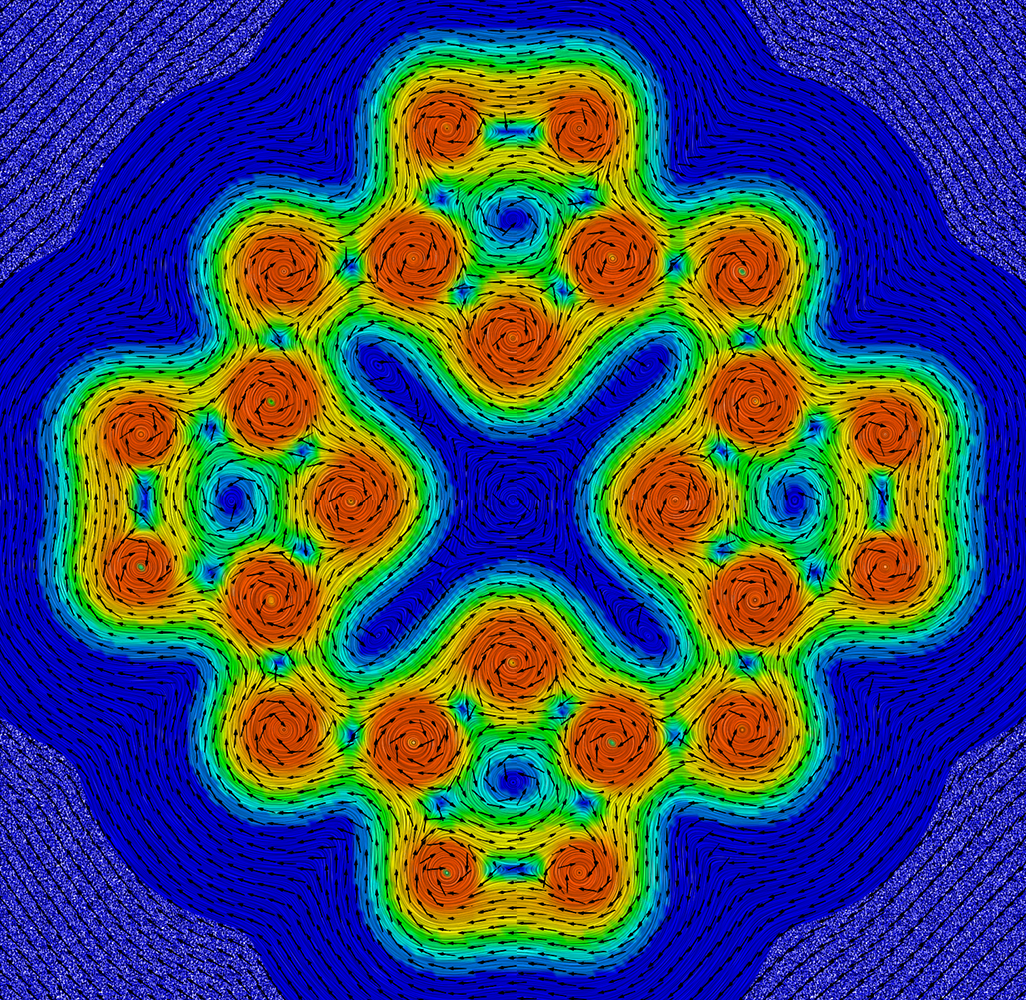
\includegraphics[width=0.6\textwidth]{hgte_1bohr}
%	\captionsetup{figurewithin = chapter}
%	\captionsetup{font=small, labelfont=bf}\caption[{Ringströme in $[$Hg$_8$Te$_8$(Te$_2$)$_4]^{8-}$}]{Ringströme in $[$Hg$_8$Te$_8$(Te$_2$)$_4]^{8-}$ \unit[1]{bohr} oberhalb der Molekülebene, dargestellt zwischen \unit[0]{a.u.} (blau) und \unit[0.07]{a.u.}.}
%\label{abb:hgtelic}
%\end{figure}
%
%\begin{figure}[ht!]
%	\centering
%	\includegraphics[width=0.6\textwidth]{b8s16_1bohr}
%	\captionsetup{figurewithin = chapter}
%	\captionsetup{font=small, labelfont=bf}\caption[Ringströme in B$_8$S$_{16}$]{Ringströme in B$_8$S$_{16}$ \unit[1]{bohr} oberhalb der Molekülebene, dargestellt zwischen \unit[0]{a.u.} (blau) und \unit[0.07]{a.u.}.}
%\label{abb:b8s16hlic}
%\end{figure}
%
%\begin{figure}[ht!]
%	\centering
%	\includegraphics[width=0.6\textwidth]{b8se16_1bohr}
%	\captionsetup{figurewithin = chapter}
%	\captionsetup{font=small, labelfont=bf}\caption[Ringströme in B$_8$Se$_{16}$]{Ringströme in B$_8$Se$_{16}$ \unit[1]{bohr} oberhalb der Molekülebene, dargestellt zwischen \unit[0]{a.u.} (blau) und \unit[0.07]{a.u.}.}
%\label{abb:b8se16hlic}
%\end{figure}

\FloatBarrier
\subsection{\texorpdfstring{[Co@Sn$_6$Sb$_6$]$^{3-}$}{[Co at Sn\_6Sb\_6]3-}}
\FloatBarrier
\section{Ringströme in großen ringförmigen Kohlenstoffnanoröhren}